\graphicspath{{chapters/ch-introduction/figures/}}
\chapter{Introduction}


\label{sec:introduction}

Until now, research in the sensor network domain has mainly focused on
routing, data aggregation, and energy conservation inside a single
sensor network while the integration of multiple sensor networks has
only been studied to a limited extent. However, as the price of
wireless sensors diminishes rapidly we can soon expect large numbers
of autonomous sensor networks being deployed. These sensor networks
will be managed by different organizations but the interconnection of
their infrastructures along with data integration and distributed
query processing will soon become an issue to fully exploit the
potential of this ``Sensor Internet.'' This requires platforms which
enable the dynamic integration and management of sensor networks and
the produced data streams.

The Global Sensor Networks (GSN) platform aims at providing a flexible
middleware to accomplish these goals.  GSN assumes the simple model
shown in Figure~\ref{fig:setup}. A sensor network internally may use
arbitrary multi-hop, ad-hoc routing algorithms to deliver sensor
readings to one or more sink node(s). A sink node is a node which is
connected to a more powerful base computer which in turn runs the GSN
middleware and may participate in a (large-scale) network of base
computers, each running GSN and servicing one or more sensor networks.

\begin{figure}
  \centering
  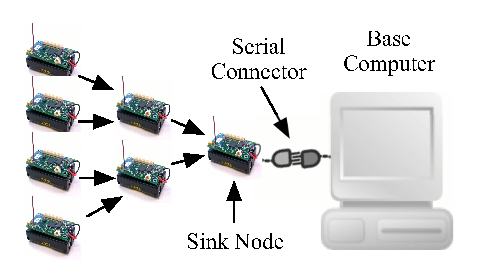
\includegraphics[width=0.5\columnwidth]{model}
  \caption{GSN model}
  \label{fig:setup}
\end{figure}

We do not make any assumptions on the internals of a sensor network
other than that the sink node is connected to the base computer via a
software wrapper conforming to the GSN API. On top of this physical
access layer GSN provides so-called \textit{virtual sensors} which
abstract from implementation details of access to sensor data and
define the data stream processing to be performed. Local and remote
virtual sensors, their data streams and the associated query
processing can be combined in arbitrary ways and thus enable the user
to build a data-oriented ``Sensor Internet'' consisting of sensor
networks connected via GSN.

\begin{comment} %following paragraph not really relevant in this context
In the following we start with a detailed description of the virtual
sensor abstraction in Section~\ref{sec:virt-sens-spec}, discuss GSN's
data stream processing and time model in
Section~\ref{sec:data-stre-proc}, and present GSN's system architecture
along with a discussion of essential implementation details
in Section~\ref{sec:system-architecture}. We
evaluate the performance of GSN in Section~\ref{sec:evaluation} and
discuss related work in Section~\ref{sec:relatedwork} before
concluding.
\end{comment}
\section{Terminology}

\begin{itemize}
	\item \textbf{Global Sensor Networks} (\gsn) defines both the project and the software described in this document. \\
	\item A \textbf{Wrapper} (\wrapper) is a piece of Java code that does the data acquisition for a specific type of device. \\
	\item A \textbf{Virtual Sensor} (\vs) is the main component in \gsn. It receives data from one or more \wrapper. It can combine their data, 
		process and finally store it. A \vs is defined in a single \vsd and combines different pieces of software 
	\begin{itemize}
		\item One \vsp
		\item Zero or Many \wrapper\textit{(s)}
	\end{itemize}
	\item A \textbf{Virtual Sensor Description file} (\vsd) is an XML file that contains the selection and the parametrization of the \vsp and \wrapper that compose a \vs.
		This file also contains the SQL statements that connect them together. \\
	\item A \textbf{Virtual Sensor Processing class} (\vsp) is a piece of Java code that process and stores the data upon reception from the \wrapper. \\
\end{itemize}

\section{Quick Start}

GSN (for Global Sensor Networks) is a software project that started in
2005 at EPFL in the LSIR Lab by Ali Salehi, under the supervision of
Prof. Karl Aberer. The initial goal was to provide a reusable software
platform for the processing of data streams generated by wireless
sensor networks. The project was successful, and was later reoriented
towards a generic stream processing platform.

GSN acquires data, filters it with an intuitive, enriched SQL syntax,
runs customisable algorithms on the results of the query, and outputs
the generated data with its notification subsystem.

GSN can be configured to acquire data from various data sources. The
high number of data sources in GSN allows for sophisticated data
processing scenarios. In the unlikely event that your data sources are
not supported, it is very easy to write a wrapper to make your hardware
work with GSN (you can find more information about this in chapter 5).

GSN offers advanced data filtering functionalities through an enhanced
SQL syntax. It is assumed that the reader has some knowledge of the
Standard Query Language (SQL). Using it for basic operations is fairly
intuitive and you should be able to start using it from the examples
provided in this document.

\section{Installing GSN from binary}

Due to the quick development cycle of GSN, you should install the
latest version.  It can always be found at
\url{http://gsn.sourceforge.net/download/}.

Before installing GSN, please download the latest version (at least
version 6) of the Java Development Kit from http://www.java.com. The
default settings should be fine.

At the time of writing (14/2/2008), the version of the installer is
0.95 is dated 15/04/2007. The installer includes a Windows batch file,
gsn-win-nogui.bat and a unix shell script, gsn-unix-nogui.sh, which
will run the GSN server (com- mand line - no gui). You may need to
modify the supplied configuration file conf/gsn.xml to select the
database that you will be using. To use the in memory database ensure
that the following line is uncommented:

\begin{bashcode}[caption={Database configuration in GSN.}, label=listing:bash:dbconfig]
\texttt{\begin{math}<\end{math}storage user="sa" password="" driver="org.hsqldb.jdbcDriver" url="jdbc:hsqldb:MEM:."/\begin{math}>\end{math}}
\end{bashcode}

This version includes no tools to run the GSN graphical user interface.

\section{Installing GSN from source}

If you wish to run the most recent version of GSN (or run the GUI), then you will need to run the source code version which is available from the SVN repository at \url{http://gsn.svn.sourceforge.net/viewvc/gsn/}.

\subsection{To run from a command line}

\begin{itemize}
	\item Download the Jakarta apache ant version 1.7.x or higher.
	\item Add the full pathname to the ANT\_HOME/bin folder to your PATH
	\item Ensure you have the latest version Sun JDK installed.
	\item Download and install TortoiseSVN (for Windows) or SmartSvn (OS
independent) or a command line SVN client:
	\item svn co https://gsn.svn.sourceforge.net/svnroot/gsn/trunk gsn
	\item Check out the GSN source code from link -
\url{https://gsn.svn.sourceforge.net/svnroot/gsn}
\end{itemize}

\setlength{\tymin}{10pt}
\setlength{\tymax}{0.8\textwidth}
\begin{table*}[!htp] 
\centering
{\normalfont\footnotesize
\begin{tabulary}{\textwidth}{|C|J|}%{|p{41pt}|p{404pt}|}
\hline

Task
 & 
Name Description
 \\
\hline

gsn
 & 
Starts the GSN server.
 \\
\hline

restart
 & 
Stops any running GSN server and starts it again.
 \\
\hline

stop
 & 
Stops the currently runing GSN server.
 \\
\hline

gui
 & 
Starts the GSN graphical user interface.
 \\
\hline

jar
 & 
Creates a jar \_le from the source.
 \\
\hline

clean
 & 
Removes the current build files and forces a rebuild. You may need to
run this task once you TODO Something missing in existing pdf
 \\
\hline

cleandb
 & 
Removes the redundant tables which are create for holding GSN's
internal states.
 \\
\hline
\end{tabulary}
}\caption{List of Ant tasks for GSN.}
%\label{table:gsn_ant_tasks} duplicate label removed)
\end{table*}

To run any of the aforementioned ant tasks simply write: ant task\_name.

\subsection{Installing to Run and debug GSN in Eclipse.}

The GSN code can also be installed to run and debug in the Eclipse
environment.

\begin{itemize}
	\item Download and install Eclipse SDK
	\item Start Eclipse;
	\item Download and install the Subclipse\footnote{This guide works for Eclipse 3.2, for Eclipse 3.4 the steps have changed slightly.}
(\url{http://subclipse.tigris.org/install.html});
	\item File -\begin{math}>\end{math} Import -\begin{math}>\end{math} Other
-\begin{math}>\end{math} Checkout Projects from SVN;
\begin{itemize}
	\item Check \textquotedblleft{}Create a new repository
location\textquotedblright{};
	\item Paste the repository location
\textquotedblleft{}https://gsn.svn.sourceforge.net/svnroot/gsn\textquotedblright{};
	\item Select \textquotedblleft{}trunk\textquotedblright{} and click
\textquotedblleft{}Next\textquotedblright{};
	\item Select \textquotedblleft{}Check out project configured using the New
Projects Wizard\textquotedblright{} and click
\textquotedblleft{}Finish\textquotedblright{};
	\item In the New Projects Wizard select \textquotedblleft{}Java
Project\textquotedblright{} and click
\textquotedblleft{}Next\textquotedblright{};
	\item In the New Java Projects Wizard
\begin{itemize}
	\item enter the project name, select \textquotedblleft{}Create new project
in workspace
	\item select \textquotedblleft{}Create separate folders
\ldots{}\textquotedblright{} and click on \textquotedblleft{}Configure
default:
	\item if the project doesn't contains a \textquotedblleft{}src\textquotedblright{} directory (depends on the Eclipse version you are using), assure to create one by
		clicking on the \textquotedblleft{}Create new source folder\textquotedblright{}
	\item In Build Path preferences select
\textquotedblleft{}Folders\textquotedblright{}, enter
\textquotedblleft{}build/classes\textquotedblright{} as the output
folder name and click \textquotedblleft{}OK:'
	\item click \textquotedblleft{}Finish\textquotedblright{};
\end{itemize}

	\item Click \textquotedblleft{}Ok\textquotedblright{} to confirm overwrite
of non standard resources;
	\item Wait for the files to download from the repository;
\end{itemize}

	\item To add library files to the build path:
\begin{itemize}
	\item Project -\begin{math}>\end{math} Properties
	\item In the Properties dialog select \textquotedblleft{}Java Build
Path\textquotedblright{};
	\item In the Java Build Path dialog, select the
\textquotedblleft{}Libraries\textquotedblright{} tab
	\item On the Libraries tab, click on \textquotedblleft{}Add jars
\ldots{}\textquotedblright{};
	\item Add only the .jar files in the lib directory and its subfolders.
\end{itemize}

\end{itemize}

GSN is now ready to Run.

Refer also to the \textquotedblleft{}How to Install Eclipse, Subclipse
and GSN, Step-by-step walkthrough\textquotedblright{} on the GSN
documentation page at: http://gsn.sourceforge.net/documentation/.

\subsection{Configuring eclipse to run/debug GSN through Eclipse.}

\textbf{Step 1: Setting the Ant Home :}

\begin{itemize}
	\item Download the Ant binaries (apache-ant-1.7.x-bin.zip) from
\url{http://ant.apache.org/};
	\item Extract the folder apache-ant-1.7.x to a suitable location on your
hard drive;
	\item Open Eclipse and do the following steps to set the Ant Home:
\begin{itemize}
	\item Go to Window Menu and select Preferences, on the left side, click on
ANT and then select Runtime.
	\item In the Classpath tab (opened on the center of the window) select Ant
Home Entries, click on the Ant Home button and browse toward the
directory that contains the files from the jakarta-ant archive
(\textbackslash apache-ant-1.7.x\textbackslash bin).
	\item Click on OK in the Browse window and again to exit the Preferences
dialog.
\end{itemize}
\end{itemize}

\textbf{Step 2: Setting an Ant Build System for your GSN project :}

\begin{itemize}
	\item Select the GSN project and on the Project menu click on properties
tab.
	\item On the Properties sheet for the project, select Builders on the left
side and click on \textquotedblleft{}New\textquotedblright{} and select
\textquotedblleft{}Ant Builder\textquotedblright{}.
	\item A \textquotedblleft{}Builder Properties for
\ldots{}\textquotedblright{} window pops up which has several tabs :
\begin{itemize}
	\item Main Tab :
\begin{itemize}
	\item For build file, click on Browse Workspace and select the build.xml
file
	\item For base directory, click on the Browse Workspace and click on the
project name which contains the gsn source code.
	\item Leave the \textquotedblleft{}Set an Input Handler\textquotedblright{}
selected.
\end{itemize}

	\item Targets Tab :
\begin{itemize}
	\item For After a Clean, click on Set Targets and select both Build and
Bind.
	\item Click on Ok.
\end{itemize}

	\item Back in the Builders page
\begin{itemize}
	\item Select the new Ant Builder
	\item De-select the existing Java Builder and click OK in the confirmation
panel which will appear.
	\item Move the new Ant Builder to the top of the list.
\end{itemize}

	\item Click on OK.
\end{itemize}

\end{itemize}

\subsection{Trying it out}

\begin{itemize}
	\item Build the project.
	\item Set the gsn-controller-port parameter:
\begin{itemize}
	\item Open build.xml, locate the gsn-controller-port value and copy it to
the clipboard;
	\item Open the Run dialog (Run -\begin{math}>\end{math} Open Run Dialog
\ldots{});
	\item In the target Run Configuration (eg. Main):
\begin{itemize}
	\item Go to the \textquotedblleft{}Arguments\textquotedblright{} tab;
	\item Paste or type the gsn-controller-port value from build.xml;
	\item Click \textquotedblleft{}Close\textquotedblright{}
\end{itemize}

	\item Click on the Run button on the toolbar
	\item The GNS application should display \textquotedblleft{}GSN Starting
\ldots{}\textquotedblright{} in the console;
	\item Open a web browser and browse to \url{http://localhost:22001} and
verify that the GSN server is working.
	\item Stop the running GSN using the ant Stop task;
	\item Insert a breakpoint in the first line of the Main class;
	\item Start the application from the
\textquotedblleft{}Debug\textquotedblright{} button on the Eclipse
toolbar;
	\item GSN should start in the Eclipse Debug perspective and pause at the
breakpoint;
\end{itemize}

\end{itemize}

Now you can debug your virtual sensors in eclipse, try it by setting a
break point on a line in the main file.



